%` `%
\def\sectionabstract{测试简介}
%\section{概述}

%本手册主要提供HPM1000微控制器的功能介绍,主要特性和设计指标。\par
%本产品是一款超高性能通用微控制器,以RISC-V双核CPU为系统电源,主频达700 MHz,提供高达2 MB的片上SRAM存储器,丰富的外设:视频音频系统,信息安全模块,外部存储接口,定时器和高性能PWM,通信接口,模拟外设和完整的时钟和电源管理系统。本产品主要面向工业控制,智能家居,人机界面,马达控制,医疗电子,语音识别,数字信号处理和人工智能等多领域应用。

%\bookmark[rellevel=0, dest=secintro]{Test}
%\clearpage
%\hypertarget{secintro}{}%
%\bookmark[level=0, dest=secintro]{产品概述}
\section{测试项目介绍} 
本文的介绍的测试项目如\autoref{tbl:appsum}:\par

\begin{center}    

    \begin{longtable}{|>{\raggedright\arraybackslash}m{3.5cm}
        |>{\raggedright\arraybackslash}m{10.5cm}
        |>{\raggedright\arraybackslash}m{3.5cm}|}
        \hline
		\textbf{测试项}    & \textbf{功能描述} \\\endhead
	\hline
    Fuse的读取 & 读取芯片的FUSE值数据,并将数据存放到EXCEL表格中 \\
    \hline
    基本功能验证 &  运行HelloWorld工程,检查芯片的JTAG调试,串口打印是否正常 \\
    \hline    
    温度传感器验证 &  运行TSNS例程,检查芯片的温度校准是否正常\\
	\hline	
    IRC24M验证 &  运行晶振测试例程,检查芯片的IRC24M是否精准,误差不超过1%\\
	\hline	
    \caption{测试项目简介}
    \label{tbl:appsum}
    \end{longtable}
\end{center}

%\begin{itemize}
%    \item RISC-V处理器本地存储器使用限制
%    \item 随机数发生器RNG使用限制
%    \item 显示接口LCDC场同步VSYNC中断/状态标志使用限制
%    \item 侵入检测模块TAMP使用限制
%    \item 模数转换器ADC12、ADC16的CONT\_EN控制位使用限制
%\end{itemize}


\clearpage
\subsection{Fuse的读取}
\subsubsection{环境搭建}
硬件:准备好芯片相应的SOCKET板子,将芯片放入SOCKET,使用TYPEC线插入UART口或者USB口,连接到PC。将拨码开关调整到BOOT0=0,BOOT1=1,按下RESET键。\par
软件:电脑下载HPMicro Manufacturing Tool,将压缩包文件解压既可:%\hypertarget{https://gitee.com/hpmicro/hpm\_sdk}
\href{\\192.168.11.200\\Shared\\HPM\_SDK\tools\hpm\_manufacturing\_tool}{NAS地址} \\	
%\\192.168.11.200\Shared\HPM_SDK\tools\hpm_manufacturing_tool。\par

\subsubsection{连接到工具}
打开下载好的HPMicro Manufacturing Tool,在解压出来的文件夹下打开这个GUI,如\autoref{fig:GUIopen}所示:\par
\vspace{\baselineskip}
\vspace{0.4cm}
\begin{figure}[H]
	\centering
	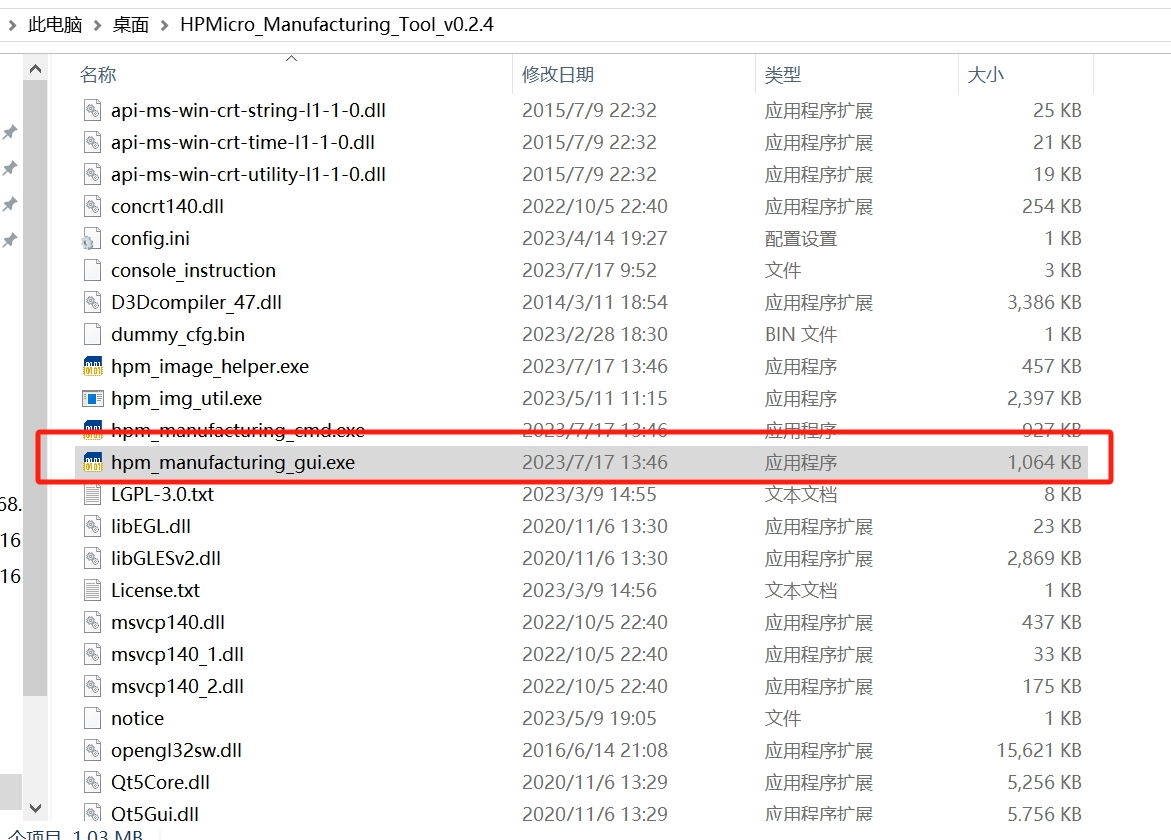
\includegraphics[width=0.7\linewidth]{img/GUIopen}
	\caption{}
	\label{fig:GUIopen}
\end{figure}

\vspace{\baselineskip}
\vspace{0.5cm}  

打开HPMicro Manufacturing Tool之后,根据TYPEC线插入的是UART口还是USB口,选择相对应的连接方式并选择插入的电脑COM端口,注意此时这个COM端口不能被其他串口工具占用。\par
如果芯片正常,BOOTPIN拨码是01,那么点击连接就可以连接上HPM烧录工具了。如果连接不上,可以试试重新上电。\par
连接成功如\autoref{fig:ConnectGUI}所示:\par
\vspace{\baselineskip}
\vspace{0.4cm}
\begin{figure}[H]
	\centering
	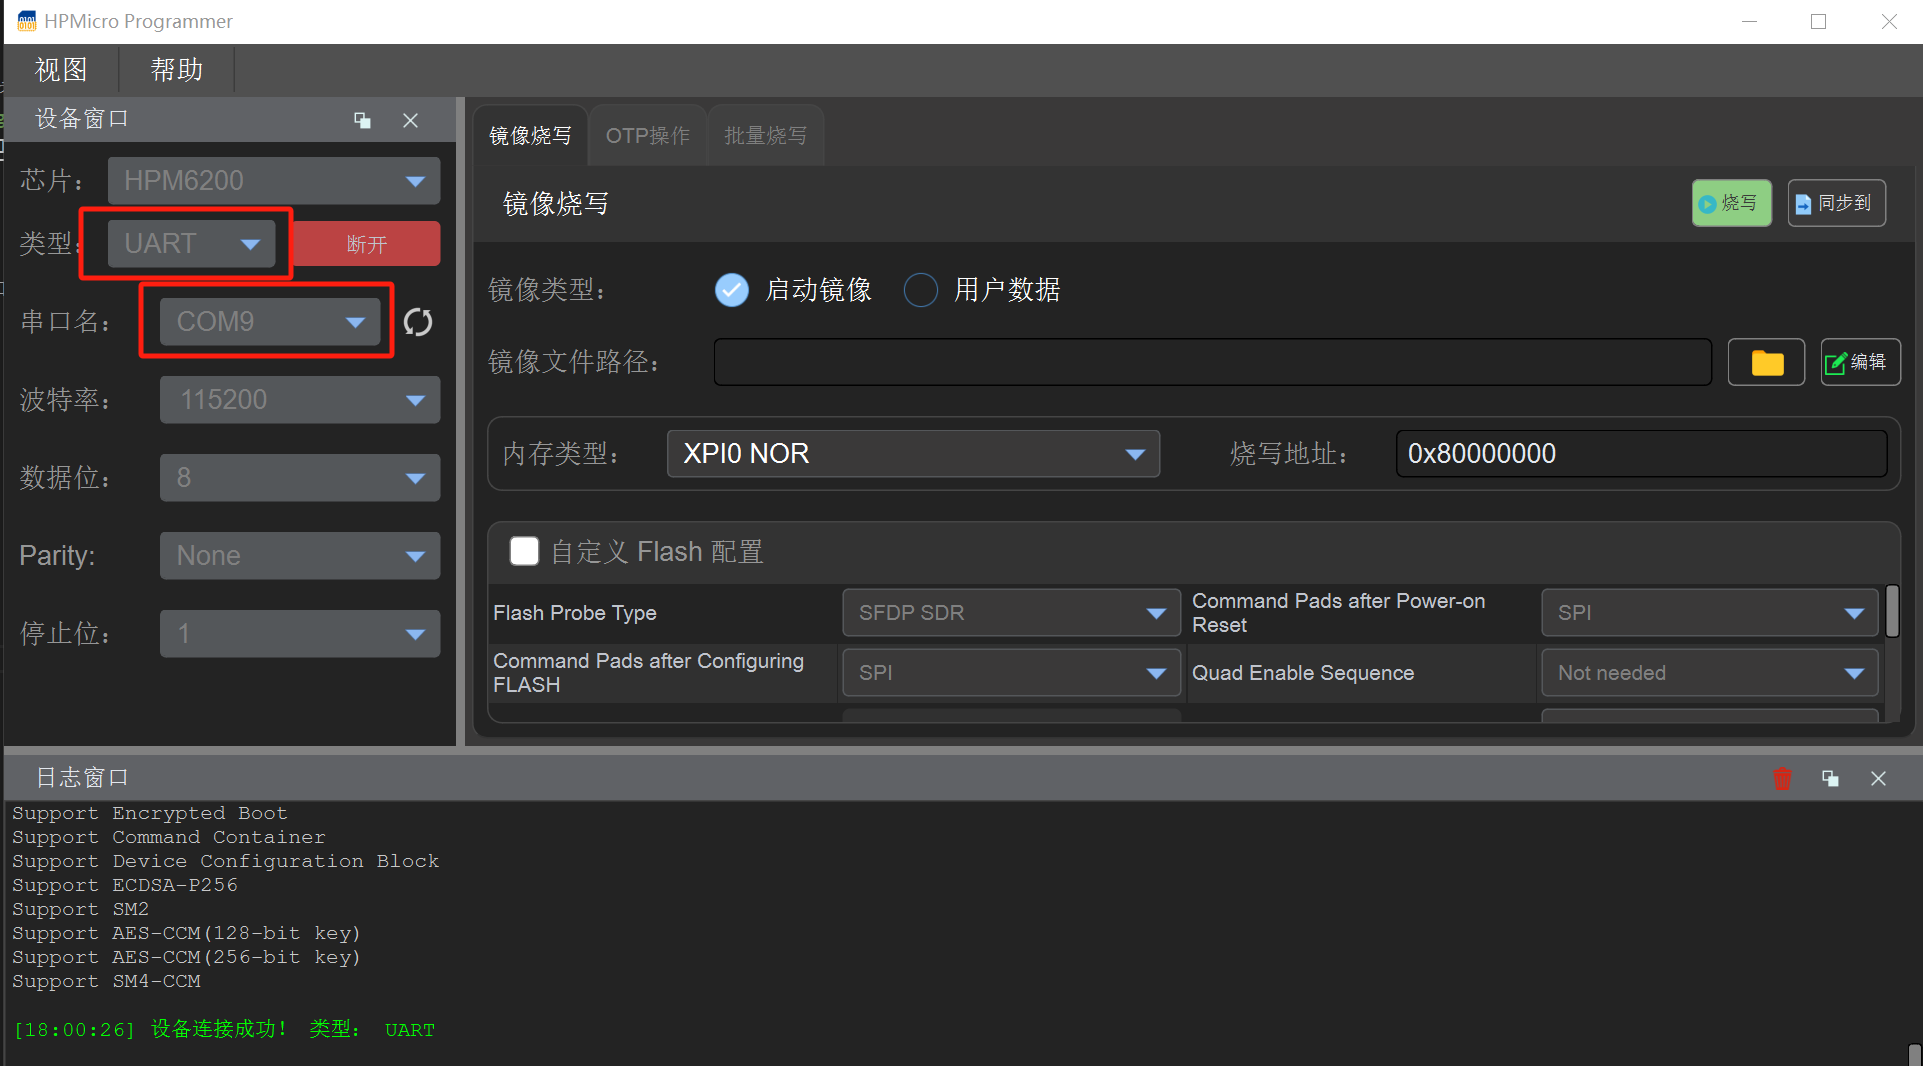
\includegraphics[width=0.7\linewidth]{img/ConnectGUI}
	\caption{}
	\label{fig:ConnectGUI}
\end{figure}

\vspace{\baselineskip}
\vspace{0.5cm} 


\subsubsection{读取FUSE值}
连接成功之后,就可以顺利读取FUSE值,点击OTP操作并刷新,就可以在工具中看到此芯片的FUSE值。点击导出就可以将EXCEL格式保存下来了。\par
读取成功如\autoref{fig:GetFuse}所示:\par
\vspace{\baselineskip}
\vspace{0.4cm}
\begin{figure}[H]
	\centering
	\includegraphics[width=0.9\linewidth]{img/GetFuse}
	\caption{}
	\label{fig:GetFuse}
\end{figure}

\vspace{\baselineskip}
\vspace{0.5cm} 

\clearpage
\subsection{基本功能验证}
\subsubsection{环境搭建}
硬件:准备好芯片相应的SOCKET板子,将芯片放入SOCKET,使用TYPEC线插入UART口,将野火cmsis\_dap调试器连接到JTAG。\par
软件:安装好SEGGER。下载SDK\_ENV包,解压到自定义路径下,这个路径不能有中文和空格等特殊字符。建议全英文。\par
安装任意一款串口工具,以此来看打印信息,本文下载SSCOM工具为例,如\autoref{fig:sscom}所示:\par
连接好SOCKET板子之后,选择CH340后缀的com口,并点击打开串口按钮。
\vspace{\baselineskip}
\vspace{0.3cm}
\begin{figure}[H]
	\centering
	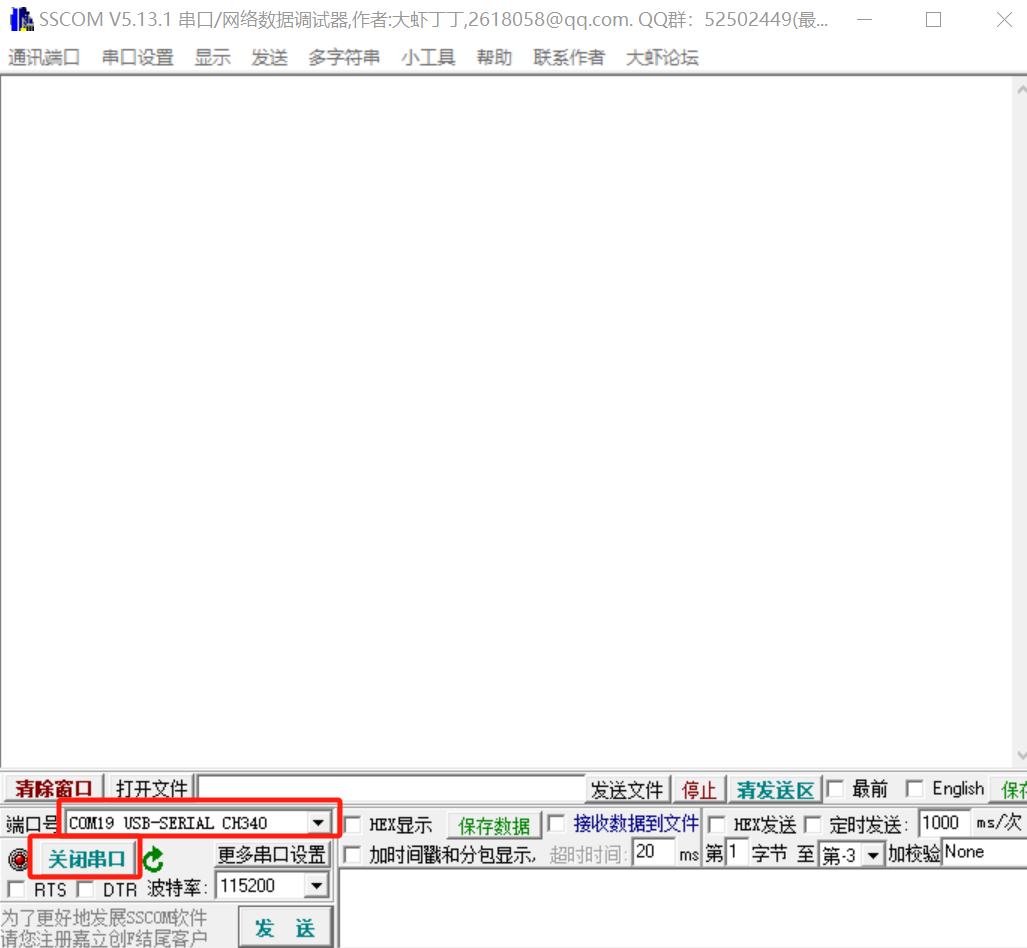
\includegraphics[width=0.7\linewidth]{img/sscom}
	\caption{}
	\label{fig:sscom}
\end{figure}
\vspace{\baselineskip}
\vspace{0.3cm} 



\subsubsection{运行HelloWorld工程}
在SDK的路径下,双击打开start\_gui.exe,根据芯片的型号,选择相对应的SDK Board,同时选择hello\_world例程进行创建,这里以HPM6200为例,如\autoref{fig:helloworld}所示:根据图中顺序依次选择,最后就会打开一个SEGGER工程。\par
\vspace{\baselineskip}
\vspace{0.3cm}
\begin{figure}[H]
	\centering
	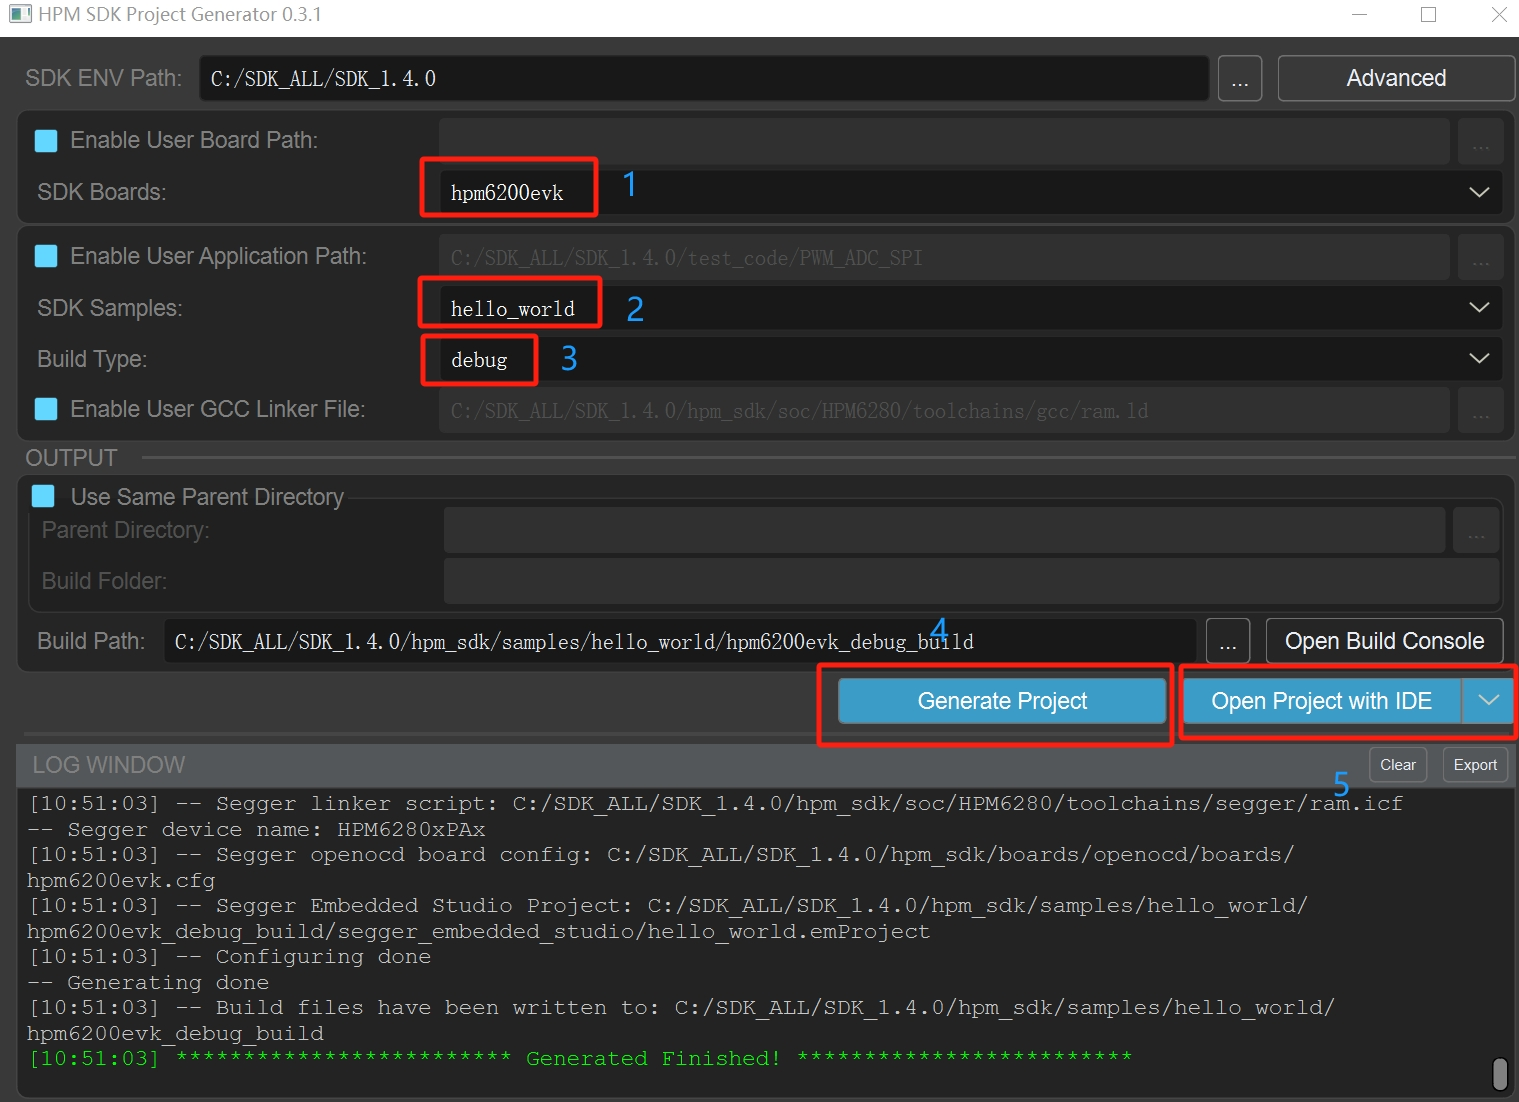
\includegraphics[width=0.7\linewidth]{img/helloworld}
	\caption{}
	\label{fig:helloworld}
\end{figure}

\vspace{\baselineskip}
\vspace{0.5cm} 

\subsubsection{工程配置}
SEGGER打开之后,需要修改一个配置,ALT+ENTER一起按下,会弹出一个选项界面,根据图中顺序依次选择,如\autoref{fig:option}所示:\par
\vspace{\baselineskip}
\vspace{0.2cm}
\begin{figure}[H]
	\centering
	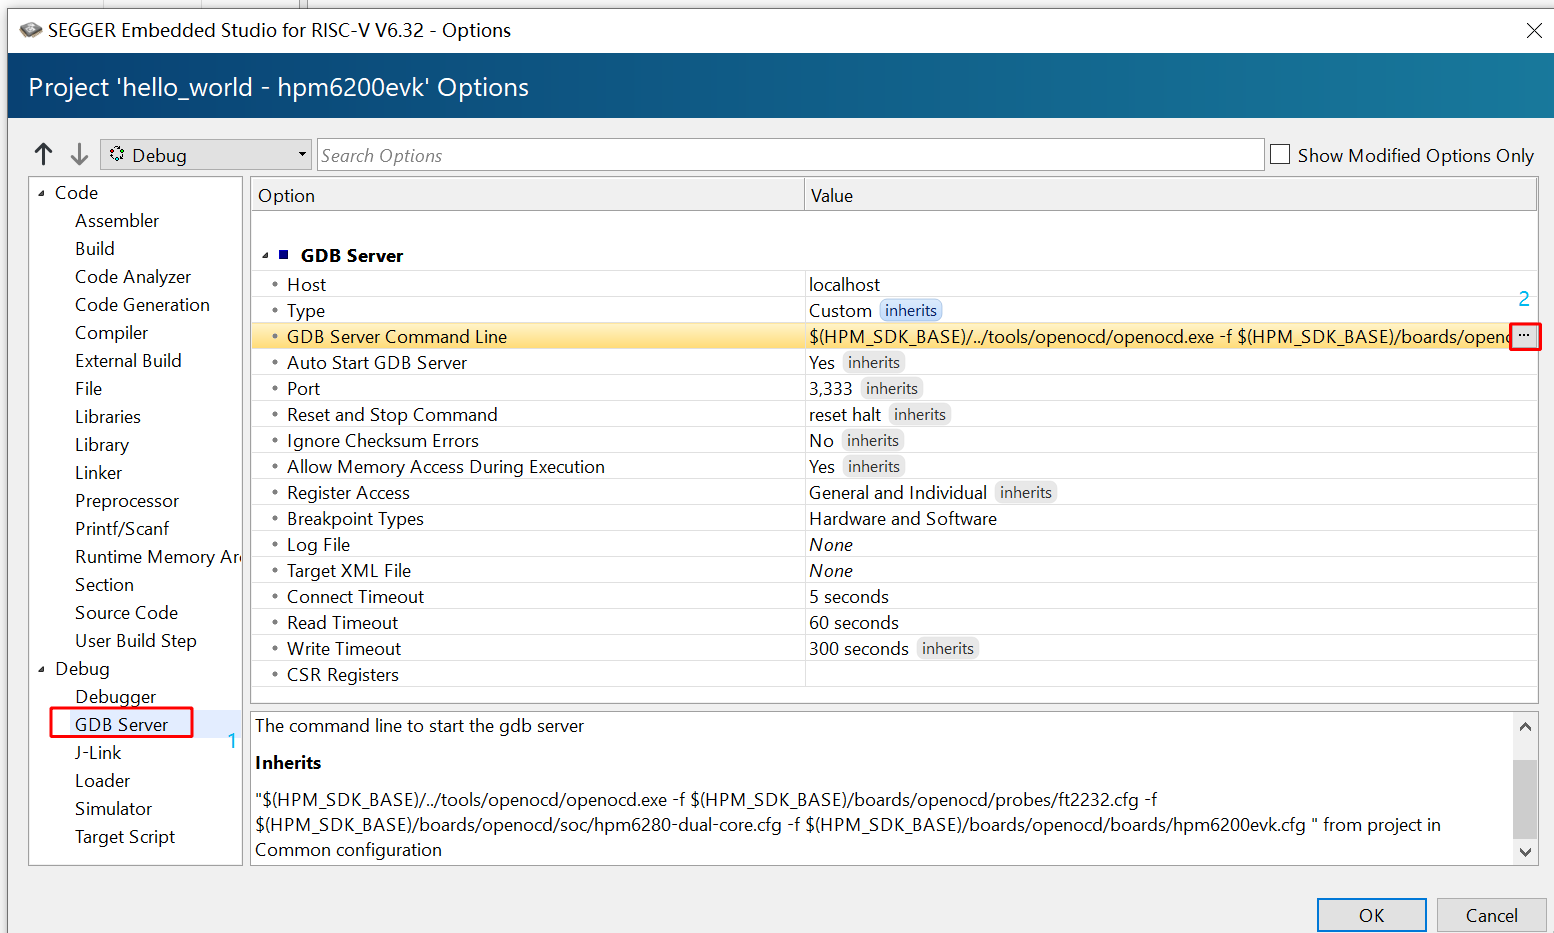
\includegraphics[width=0.7\linewidth]{img/option}
	\caption{}
	\label{fig:option}
\end{figure}

\vspace{\baselineskip}
\vspace{0.2cm} 
这样会打开详细的GDB命令,如\autoref{fig:commandline}所示:\par
\vspace{\baselineskip}
\vspace{0.2cm}
\begin{figure}[H]
	\centering
	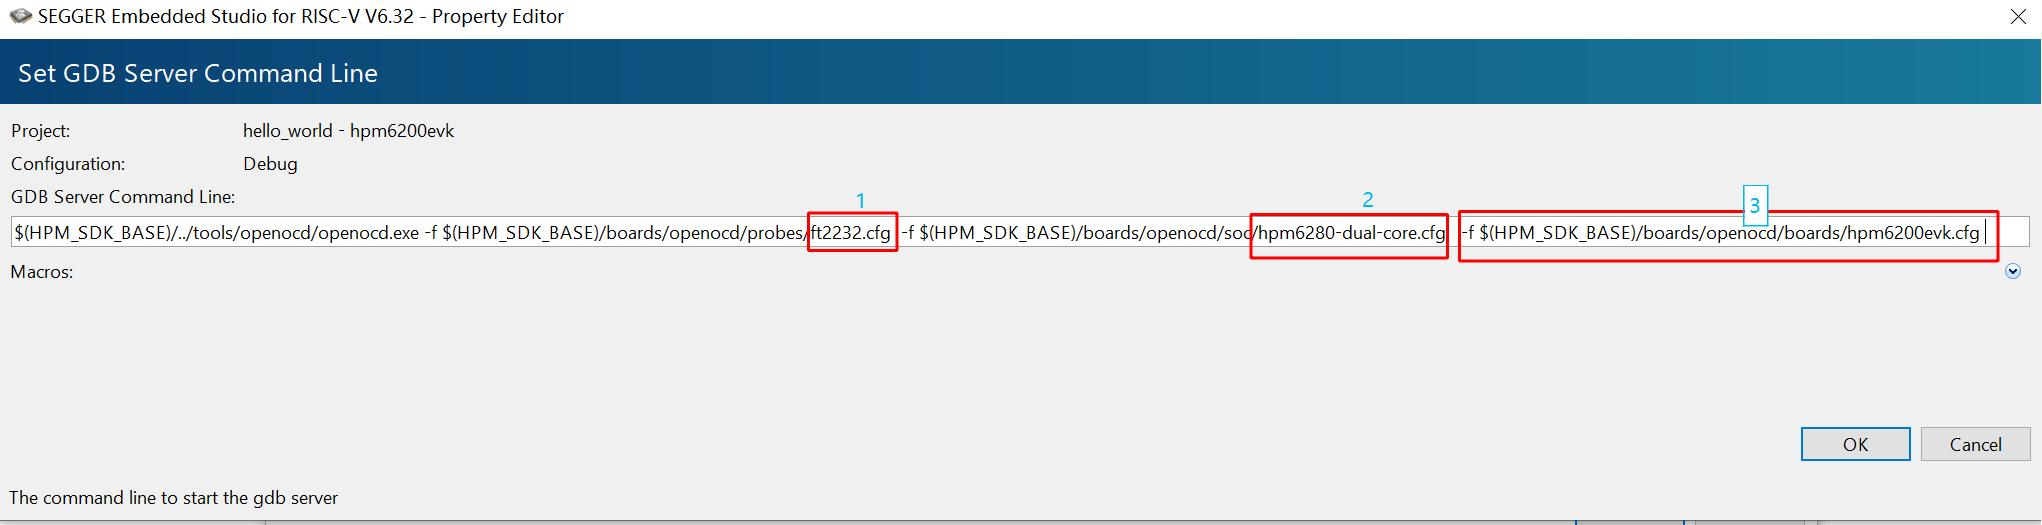
\includegraphics[width=1\linewidth]{img/commandline}
	\caption{}
	\label{fig:commandline}
\end{figure}
\vspace{\baselineskip}
\vspace{0.3cm} 

本文以HPM6200为例,如图中三处标注,这三处配置需要注意:\par
\begin{enumerate}
    \item  如果使用野火的调试器,需要将ft2232.cfg改为cmsis\_dap.cfg
    \item  如果是62双核,无需更改;如果是62单核,需要将dual改为single。如果是63本来就是单核的片子,此处可以使用默认配置,无需更改
    \item 将最后的: %\begin{lstlisting} [language=C, caption=GDB command line]
        -f \$(HPM\_SDK\_BASE)/boards/openocd/boards/hpm6200evk.cfg 
        这一段-f开始的命令给删除掉。 % \end{lstlisting} 删除掉。
\end{enumerate}

\subsubsection{运行程序}
保存好上节的配置后,点击F7编译代码,编译结束后,点击F5运行程序。或者分别点击SEGGER上方的BUILD与DEBUG-GO也可。\par
运行成功后,点击\autoref{fig:debug}的运行按键,全速运行程序:\par
如果无法正常运行程序,或者点击F5后无法进入到图中的界面,可以重新上电几次尝试,还是不行就需要检查片子是否正常了。\par
\vspace{\baselineskip}
\vspace{0.3cm}
\begin{figure}[H]
	\centering
	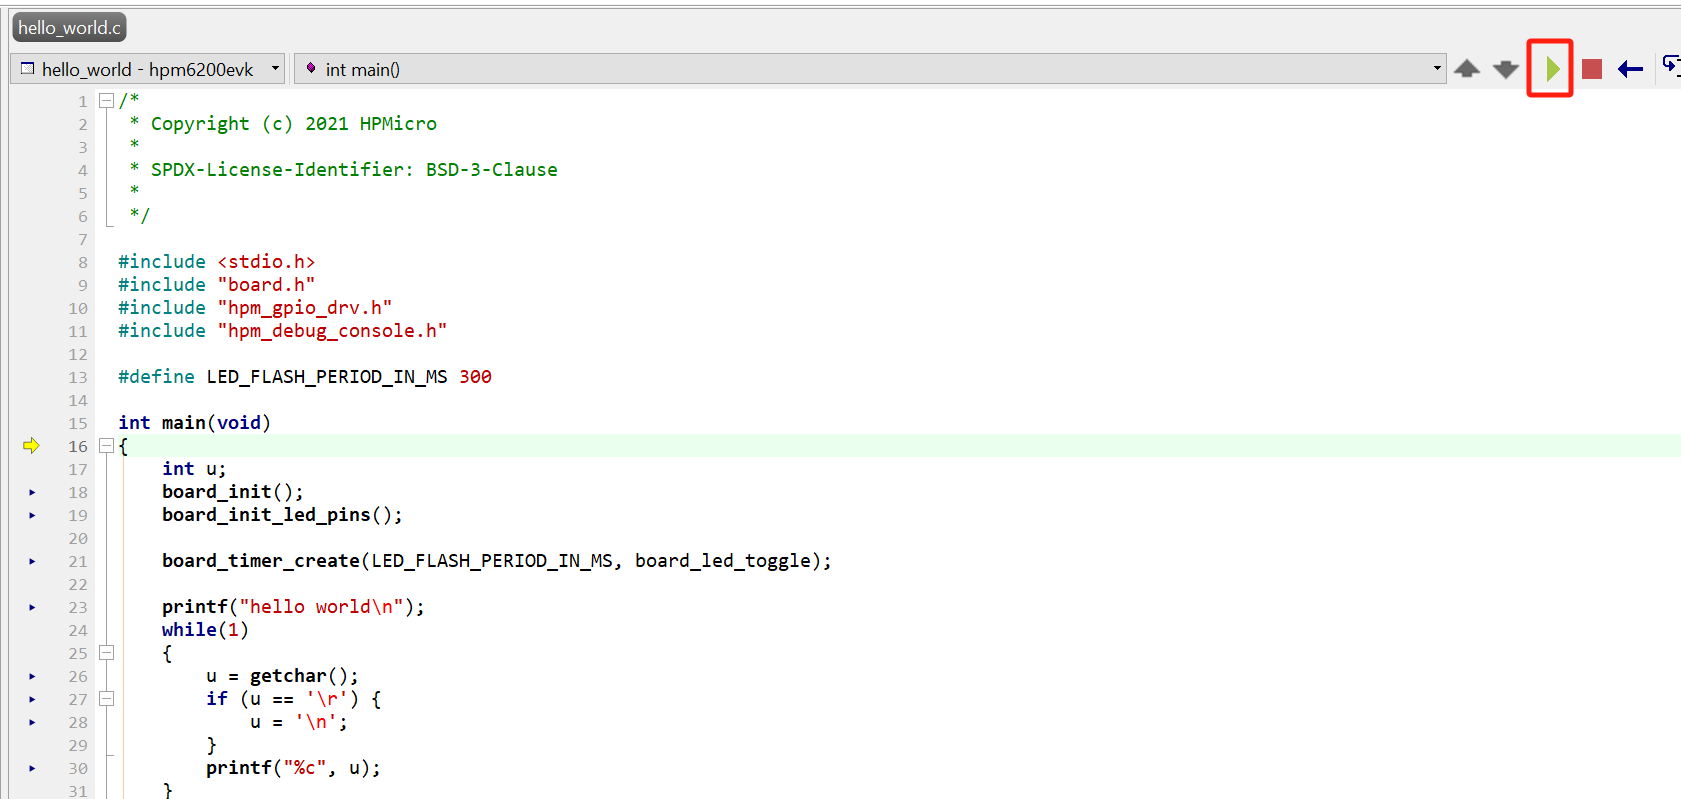
\includegraphics[width=0.7\linewidth]{img/debug}
	\caption{}
	\label{fig:debug}
\end{figure}

\vspace{\baselineskip}
\vspace{0.3cm} 

芯片如果正常工作的情况下,按下运行之后,可以在串口工具中看到打印出来的信息,helloworld,并且输入任意字符发送出去,可以在工具中看到回显,如\autoref{fig:runhello}所示:\par
\vspace{\baselineskip}
\vspace{0.2cm}
\begin{figure}[H]
	\centering
	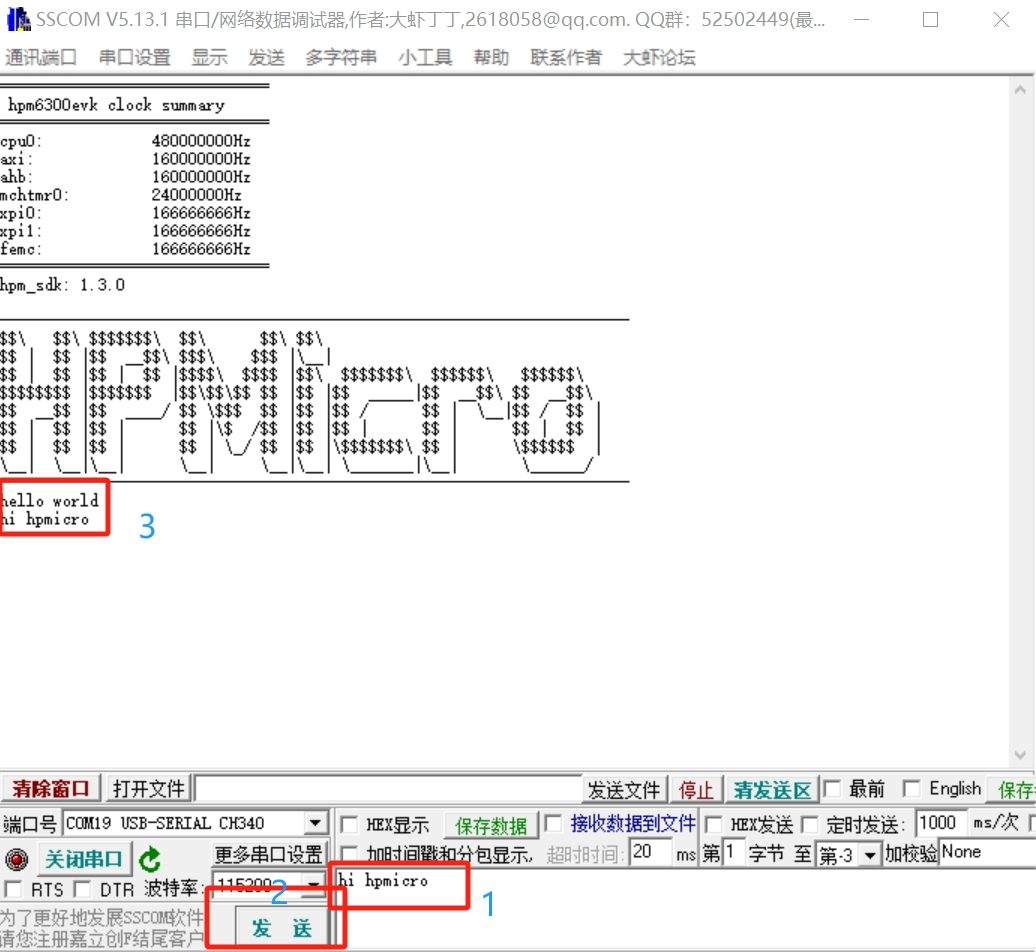
\includegraphics[width=0.7\linewidth]{img/runhello}
	\caption{}
	\label{fig:runhello}
\end{figure}
\vspace{\baselineskip}
\vspace{0.3cm} 

\clearpage
\subsection{温度传感器验证}
\subsubsection{环境搭建}
与1.2章节中helloworld的搭建基本一致,唯一有区别的地方就是GUI生成工程时,选择一下测试温度的例程,如\autoref{fig:tsns}所示:\par
\vspace{\baselineskip}
\vspace{0.2cm}
\begin{figure}[H]
	\centering
	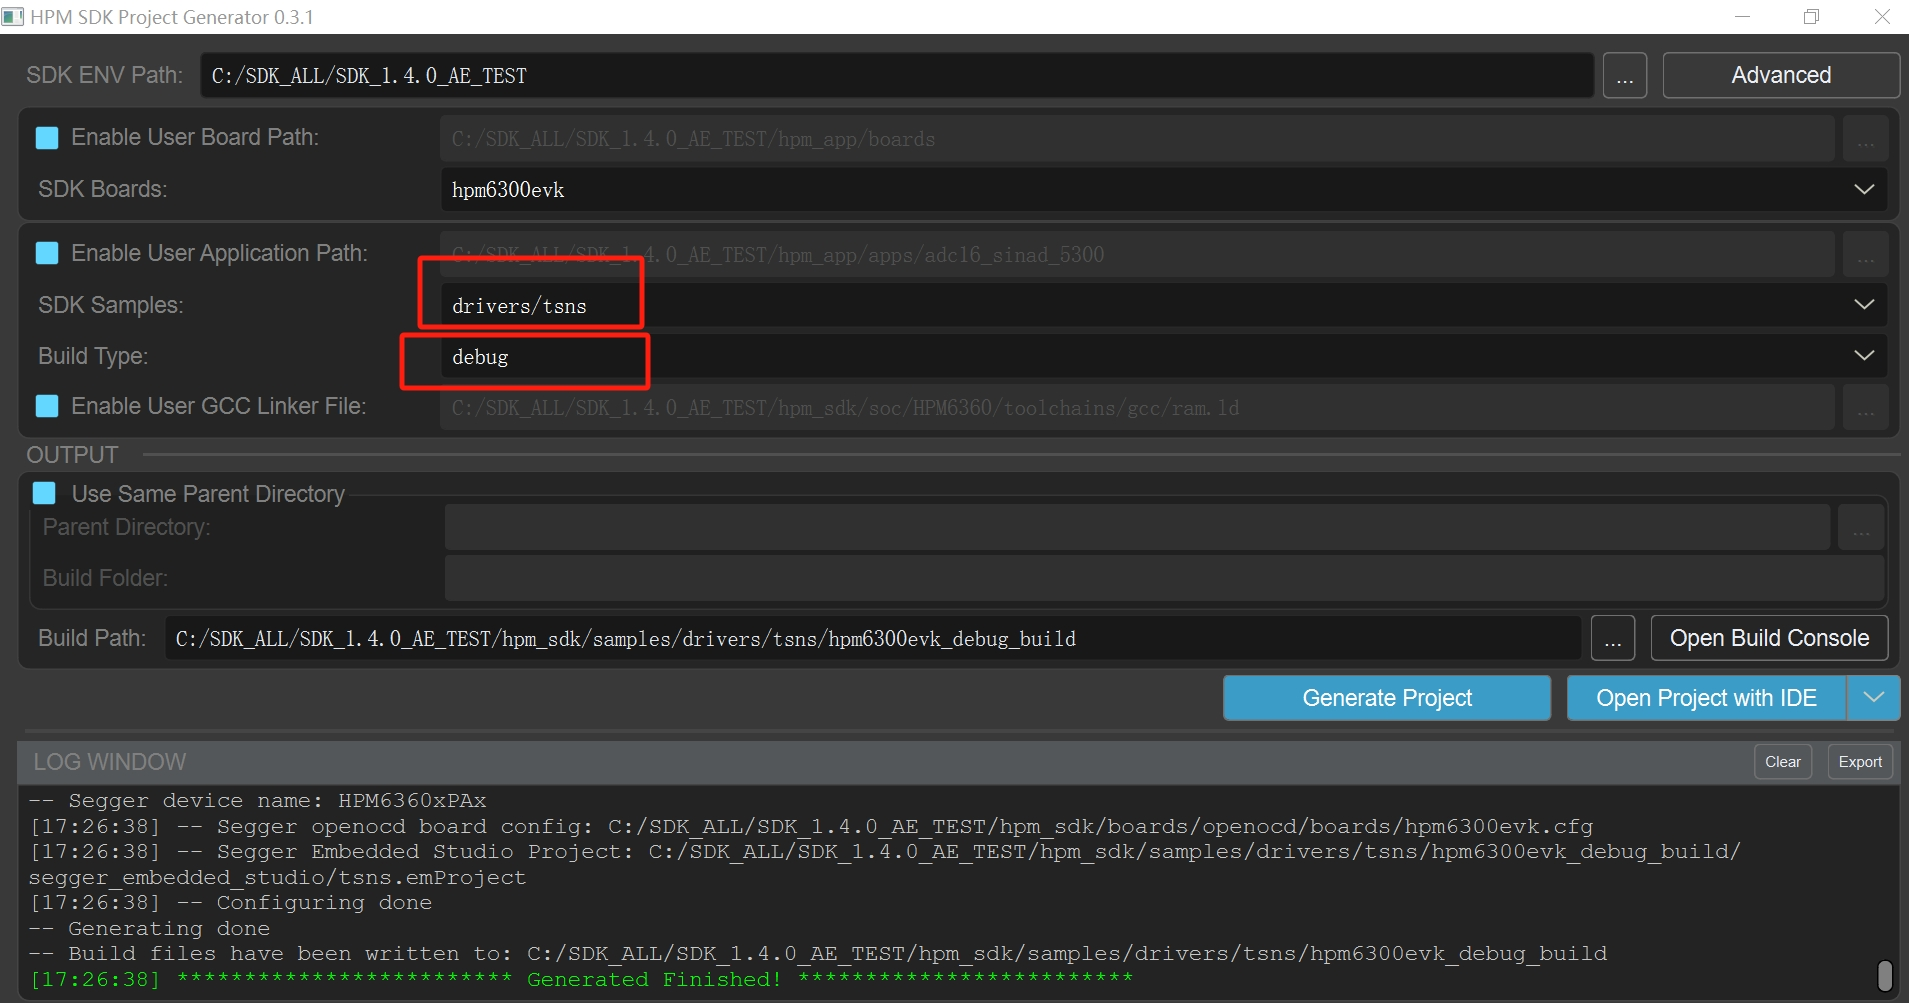
\includegraphics[width=1\linewidth]{img/tsns.png}
	\caption{}
	\label{fig:tsns}
\end{figure}
\vspace{\baselineskip}
\vspace{0.3cm} 

\subsubsection{工程配置}
与1.2章节中helloworld的搭建完全一致,修改选项中的GDB命令并运行程序。\par

\subsubsection{运行程序}
芯片如果正常工作的情况下,按下运行之后,可以在串口工具中看到打印出来的温度信息,温度会随着程序运行的时间增多,正常上升。\par
如\autoref{fig:runtsns}所示:\par
\vspace{\baselineskip}
\vspace{0.2cm}
\begin{figure}[H]
	\centering
	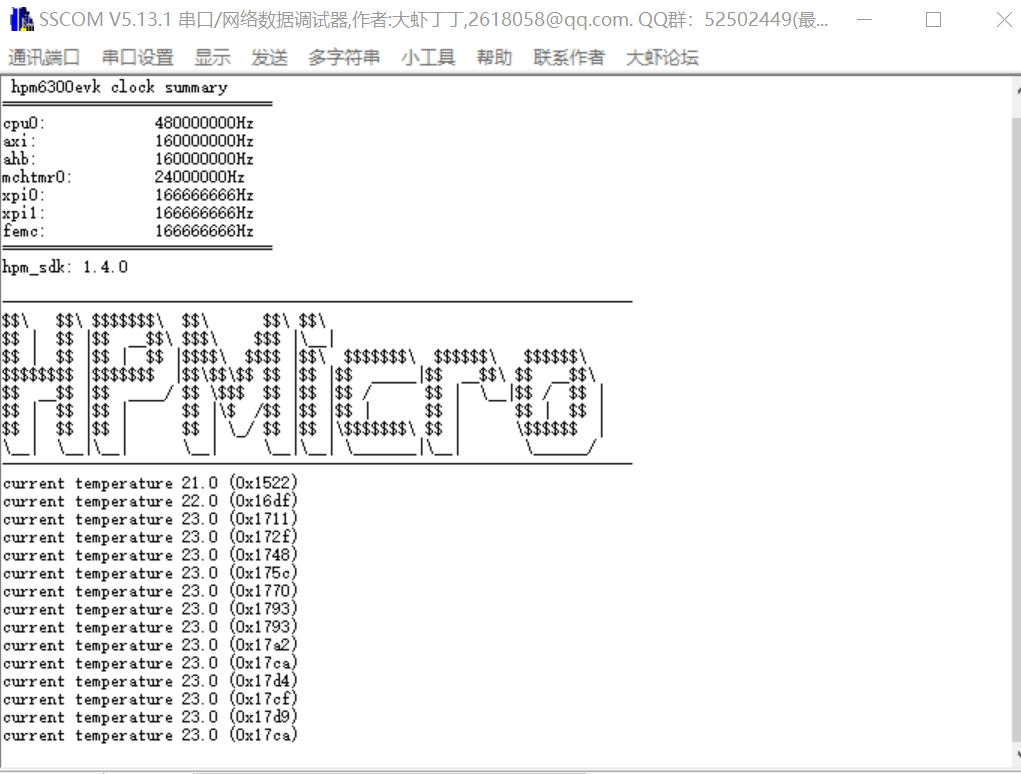
\includegraphics[width=0.7\linewidth]{img/runtsns.png}
	\caption{}
	\label{fig:runtsns}
\end{figure}
\vspace{\baselineskip}
\vspace{0.3cm} 


\clearpage
\subsection{IRC24M的精度验证}
\subsubsection{环境搭建}
与1.2章节中helloworld的搭建基本一致,唯一有区别的地方就是GUI生成工程时,选择一下测试晶振的工程。\par

\subsubsection{工程配置}
与1.2章节中helloworld的搭建完全一致,修改选项中的GDB命令并运行程序。\par

\subsubsection{运行程序}
程序成功运行之后,在特定的引脚上,可以用示波器测量到相应的频率,设置下平均频率即可,本文以63的晶振测试为例:\par
 \begin{lstlisting} [language=C, caption=IRC 24M test code]
	int main(void)
{
    board_init();
	reg32_write(0xF4002420, 0x01001301);//addr,data,63xx
	HPM_IOC->PAD[IOC_PAD_PA17].FUNC_CTL = IOC_PA17_FUNC_CTL_SYSCTL_CLK_OBS_1;

}
	 \end{lstlisting}

不同信号测量的引脚有所差异,如上述代码中可以看出,需要测量PA17。\par